% !TEX root = main.tex
\section{Phương pháp đề xuất}\label{sec:method}

\subsection{Ý tưởng tổng quát}\label{sec:method:idea}

Chúng tôi tách bài toán thành ba tầng độc lập, giao tiếp với nhau qua một giao diện duy nhất là \emph{hàm thời gian qua
cạnh} $\tau(e,t)$:
\begin{enumerate}[label=(\arabic*)]
    \item \textbf{Tầng môi trường.} Đồ thị đường từ OpenStreetMap; mô hình vận tốc 24 khung giờ $V_{\text{base}}$ (vai
    trò ``dự báo''); môi trường thực $V_{\text{real}}$ có nhiễu tương quan và sự cố, tái lập được theo seed của từng truy vấn.
    \item \textbf{Tầng tác nhân ra quyết định.} Các thuật toán tìm kiếm (Dijkstra, A*, TD-Dijkstra, TD-A*), các cơ chế tái
    lập kế hoạch, dự báo GCN, định tuyến theo rủi ro và các chính sách RL. Mọi tác nhân chỉ ``nhìn thấy'' môi trường qua
    $\tau(e,t)$ của mô hình mà nó được phép biết (dự báo, dự báo cộng quan sát, hay môi trường thực đối với oracle).
    \item \textbf{Tầng đánh giá.} Mọi tác nhân được chạy trên cùng tập truy vấn kiểm tra cố định, trong cùng $V_{\text{real}}$,
    và được so sánh với oracle bằng các chỉ số thống nhất cùng kiểm định thống kê ghép cặp.
\end{enumerate}
Cách tách này cho phép thay thế từng thành phần (ví dụ thay $V_{\text{base}}$ mô phỏng bằng dự báo từ dữ liệu thật) mà
không phải viết lại thuật toán. Sơ đồ khối của toàn hệ thống được trình bày ở Hình~\ref{fig:pipeline}
(Mục~\ref{sec:method:diagram}).

\subsection{Chi tiết thuật toán / mô hình}\label{sec:method:detail}

\subsubsection{Xây dựng đồ thị từ OpenStreetMap}\label{sec:method:graph}

\textbf{Xác định ranh giới.} Ranh giới quận Hà Đông được lấy bằng dịch vụ geocode Nominatim. Do Hà Nội bỏ cấp quận từ
ngày 01/7/2025, truy vấn ``Hà Đông'' có thể chỉ trả về \emph{phường} Hà Đông mới (khoảng 9~km\textsuperscript{2}) thay vì quận
cũ (khoảng 49~km\textsuperscript{2}). Chương trình vì vậy kiểm tra diện tích vùng trả về; nếu nhỏ hơn 20~km\textsuperscript{2}
thì lần lượt dùng: hợp của 5 phường mới tạo nên quận cũ (Hà Đông, Dương Nội, Yên Nghĩa, Phú Lương, Kiến Hưng), ranh
giới đã lưu từ lần chạy trước, và cuối cùng là một hình chữ nhật bao. Vùng đệm 500~m được thêm vào để giữ các tuyến
ra/vào quận.

\textbf{Tải và làm sạch.} Mạng đường dành cho ô tô được tải qua OSMnx~\cite{boeing2017}; chương trình thử lần lượt ba máy
chủ Overpass (trong lần chạy chính thức, máy chủ chính không phản hồi và máy chủ dự phòng thứ ba đã đáp ứng), rồi lưu
bản sao cục bộ để các lần sau chạy không cần mạng. Đồ thị thô có \RawNodes{} nút và \RawEdges{} cạnh. Quá trình làm sạch
gồm: bỏ \SelfLoops{} cạnh tự vòng; gộp \ParallelEdges{} cạnh song song (giữ cạnh ngắn nhất); giữ thành phần liên thông
mạnh lớn nhất (bỏ \DroppedNodes{} nút không đi tới/đi về được). Kết quả: \NNodes{} nút, \NEdges{} cạnh, tổng chiều dài
\TotalKm{} km, chiều dài cạnh trung bình \MeanEdgeLen{} m, bậc ra lớn nhất \MaxOutDeg{} và trung bình \MeanOutDeg.

\textbf{Chuẩn hoá thuộc tính.} Thẻ \texttt{highway} được gom về năm nhóm: \emph{trunk} (gồm cả motorway), \emph{primary},
\emph{secondary}, \emph{tertiary} và \emph{residential} (gồm các loại còn lại). Chỉ \MaxspeedCoverage\% số cạnh có thẻ
\texttt{maxspeed}; các giá trị được phân tích từ nhiều định dạng (``50'', ``50 mph'', danh sách) và giá trị thiếu được điền
theo nhóm đường (trunk 60, primary 50, secondary 40, tertiary 30, residential 20 km/h). Vận tốc tự do được lấy bằng 90\%
vận tốc tối đa. Để heuristic ở các mục sau luôn chấp nhận được, chiều dài mỗi cạnh được ép không nhỏ hơn khoảng cách chim
bay giữa hai đầu mút.

\textbf{Biểu diễn CSR.} Các cạnh được sắp theo nút đầu, và các cạnh ra của nút $u$ là đoạn
\begin{equation}
\text{out}(u) = \bigl\{\,\texttt{out\_edges}[k] : \texttt{out\_ptr}[u] \le k < \texttt{out\_ptr}[u+1]\,\bigr\},
\label{eq:csr}
\end{equation}
nên việc duyệt cạnh ra là truy cập bộ nhớ liên tục, phù hợp cho cả vòng lặp Python lẫn mã biên dịch Numba. Phân bố loại
đường được cho ở Bảng~\ref{tab:tab_graph_groups} và bản đồ ở Hình~\ref{fig:graph}.

\begin{table}[!htbp]
\centering
\small
\caption{Phân bố loại đường của đồ thị Hà Đông (sau làm sạch).}
\label{tab:tab_graph_groups}
\begin{adjustbox}{max width=\linewidth}
\begin{tabular}{lrrr}
\toprule
Nhóm đường & Số cạnh & Chiều dài (km) & Tỉ lệ (\%) \\
\midrule
trunk & 291 & 44{,}4 & 4{,}7 \\
primary & 337 & 42{,}5 & 4{,}5 \\
secondary & 244 & 33{,}5 & 3{,}5 \\
tertiary & 867 & 106{,}2 & 11{,}2 \\
residential & 7205 & 717{,}9 & 76{,}0 \\
Tổng & 8944 & 944{,}5 & 100{,}0 \\
\bottomrule
\end{tabular}
\end{adjustbox}
\end{table}


\begin{figure}[H]
\centering
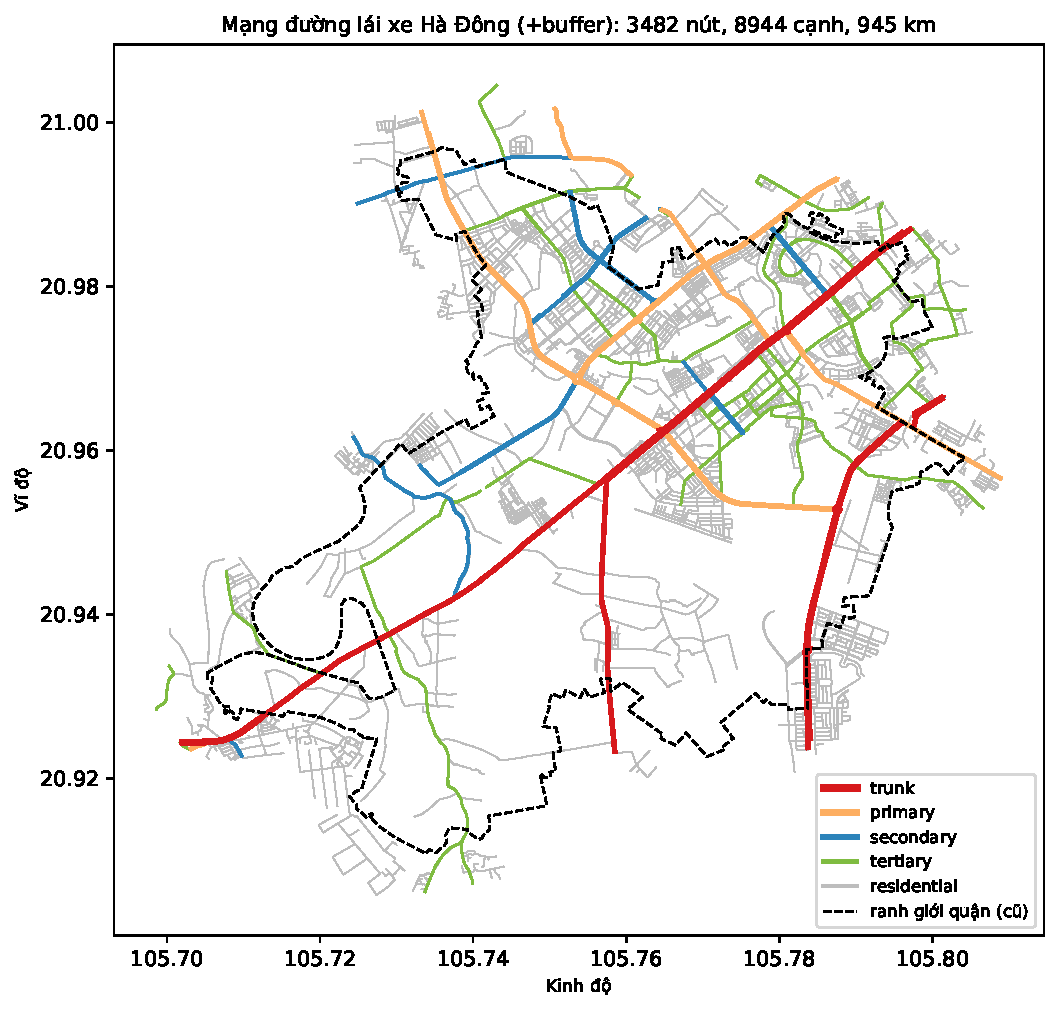
\includegraphics[width=0.72\linewidth]{graph_map.pdf}
\caption{Mạng đường lái xe quận Hà Đông (cộng vùng đệm 500 m) theo nhóm đường; nét đứt là ranh giới quận cũ.}
\label{fig:graph}
\end{figure}

\subsubsection{Mô hình vận tốc 24 khung giờ}\label{sec:method:speed}

Với mỗi cạnh $e$ và mỗi khung giờ $h\in\{0,1,\dots,23\}$, vận tốc nền được xác định bởi một \emph{mức ùn} $c(e,h)\in[0,c_{\max}]$:
\begin{equation}
v(e,h) = \max\Bigl(v_{\text{free}}(e)\bigl(1-c(e,h)\bigr),\; v_{\min}\Bigr),
\label{eq:speed}
\end{equation}
\begin{equation}
\begin{aligned}
c(e,h) = \operatorname{clip}\Bigl(\,&p(h)\cdot s(g_e)\cdot \eta(e,h)\cdot \delta(e,h) + \xi(e,h),\\
&0,\; c_{\max}\Bigr),
\end{aligned}
\label{eq:congestion}
\end{equation}
với $c_{\max}=0{,}85$ và $v_{\min}=5$ km/h. Các thành phần được thiết kế để mỗi thành phần phản ánh một hiện tượng giao
thông có thật:

\textbf{Profile theo giờ $p(h)$} là tổng các hàm Gaussian \emph{tuần hoàn} chu kỳ 24 giờ, bảo đảm tính lặp lại hằng ngày
($p(0)=p(24)$):
\begin{equation}
p(h) = b + \sum_{j} a_j \sum_{k\in\{-1,0,1\}} \exp\!\left(-\frac{(h-\mu_j+24k)^2}{2\sigma_j^2}\right),
\label{eq:profile}
\end{equation}
với các đỉnh sáng ($\mu=8$), trưa ($\mu=12{,}5$), chiều ($\mu=18$), tối ($\mu=21$) và một ``trũng'' ban đêm (biên độ âm,
$\mu=3$); tham số đầy đủ ở Phụ lục.

\textbf{Độ nhạy theo loại đường $s(g)$} phản ánh việc trục chính chịu ùn nặng hơn đường nhánh: trunk 1,0; primary 0,95;
secondary 0,8; tertiary 0,65; residential 0,4.

\textbf{Hệ số trục nóng $\eta(e,h)$} lấy từ tệp \texttt{hotspots.yaml} (Phụ lục): mỗi điểm nóng có hệ số nhân và khung giờ
ảnh hưởng; cạnh được khớp theo tên đường không dấu (loại trừ các ngõ/ngách mang tên trục), theo mã đường (ví dụ QL.6)
hoặc theo bán kính quanh toạ độ nút giao (Cầu Am, Mai Lĩnh, Bến xe Yên Nghĩa).

\textbf{Hệ số hướng $\delta(e,h)$} làm ùn nặng hơn theo hướng vào trung tâm buổi sáng và hướng ra buổi chiều:
\begin{equation}
\delta(e,h) = 1 + \beta\, a_e\,\bigl(w_{\text{sáng}}(h)-w_{\text{chiều}}(h)\bigr), \qquad
a_e = \cos\angle\bigl(\vec{e},\, \vec{c}-\vec{m}_e\bigr),
\label{eq:direction}
\end{equation}
trong đó $\vec{c}$ là toạ độ Ngã Tư Sở (tâm tham chiếu), $\vec{m}_e$ là trung điểm cạnh, $w_{\text{sáng}}, w_{\text{chiều}}$
là các Gaussian tuần hoàn quanh 8h và 18h, $\beta=0{,}3$.

\textbf{Nhiễu không gian $\xi(e,h)$} được tạo bằng cách làm mượt nhiễu Gaussian $k$ lần qua ma trận kề cạnh--cạnh chuẩn
hoá theo hàng $\hat{A}$ (hai cạnh kề nếu chung đầu mút), sau đó chuẩn hoá về độ lệch chuẩn $\sigma_\xi$:
\begin{equation}
\Xi^{(k)} = \hat{A}^{\,k}\,\Xi^{(0)}, \qquad \Xi^{(0)}_{e,h}\sim\mathcal{N}(0,1),
\label{eq:smooth}
\end{equation}
cộng thêm một thành phần nhỏ phụ thuộc ``seed ngày'' để mỗi ngày khác nhau nhưng vẫn cùng quy luật.

\textbf{Nội suy theo phút.} Với $t$ phút, đặt $h=\lfloor (t \bmod 1440)/60\rfloor$ và $\phi=((t\bmod 1440)-60h)/60$; vận tốc
được nội suy tuyến tính (vòng 24 giờ):
\begin{equation}
v_e(t) = (1-\phi)\,v(e,h) + \phi\, v\bigl(e,(h+1)\bmod 24\bigr).
\label{eq:interp}
\end{equation}

\textbf{Bảo đảm FIFO cho vận tốc nền.} Trong một khung giờ, nếu vận tốc tăng tuyến tính từ $v_\ell$ lên $v_u$ thì
$\tau_e(t)=L_e/v_e(t)$ giảm với tốc độ lớn nhất tại đầu mút có vận tốc thấp:
\begin{equation}
\max_t\left(-\frac{d\tau_e}{dt}\right) = \frac{L_e\,(v_u-v_\ell)}{60\,v_\ell^{2}}.
\label{eq:slope}
\end{equation}
Chúng tôi yêu cầu đại lượng này không vượt quá $\kappa=0{,}9<1$ (biên an toàn cho điều kiện \eqref{eq:fifo-deriv}).
Nếu vi phạm, vận tốc đầu mút thấp được nâng lên giá trị nhỏ nhất thoả mãn, tức nghiệm dương của
\begin{equation}
60\kappa\, x^2 + L_e\, x - L_e\, v_u = 0 \;\Longrightarrow\;
x = \frac{-L_e + \sqrt{L_e^2 + 240\kappa L_e v_u}}{120\kappa},
\label{eq:fifo-fix}
\end{equation}
và thủ tục lặp tới khi mọi đoạn thoả mãn (Bổ đề~\ref{bd:fifofix}). Với $V_{\text{base}}$ của Hà Đông, độ dốc lớn nhất
đo được là \FifoSlope{} nên không ô nào cần sửa.

\textbf{Sự cố.} Một sự cố trên cạnh $e$ bắt đầu lúc $t_s$, kéo dài $D$ phút, mức độ $\rho\in[0{,}1;0{,}4]$, nhân vận tốc
với hệ số
\begin{equation}
f(t)=\begin{cases}
1-(1-\rho)\dfrac{t-t_s}{r_{\text{in}}}, & t_s\le t<t_s+r_{\text{in}},\\[2mm]
\rho, & t_s+r_{\text{in}}\le t\le t_s+D,\\[1mm]
\rho+(1-\rho)\dfrac{t-t_s-D}{r_{\text{out}}}, & t_s+D<t<t_s+D+r_{\text{out}},\\[2mm]
1, & \text{ngược lại},
\end{cases}
\label{eq:incident}
\end{equation}
với $r_{\text{in}}=5$ phút (dốc vào) và $r_{\text{out}}=15$ phút (giải toả). Khi sự cố kết thúc, vận tốc tăng nhanh có thể
phá vỡ FIFO. Vì vậy hàm đến của cạnh bị sự cố được tính trên lưới 1 phút rồi \emph{FIFO hoá}:
\begin{equation}
\tilde{a}_e(t) = \min_{t'\ge t} a_e(t'),
\label{eq:fifoize}
\end{equation}
và nội suy tuyến tính giữa các điểm lưới. Về mặt vật lý, \eqref{eq:fifoize} tương ứng với việc xe đến cạnh sớm ``đợi''
ngầm để không về muộn hơn xe đến sau; Mệnh đề~\ref{md:fifoize} chứng minh tính FIFO tuyệt đối của kết quả.

\begin{figure}[H]
\centering
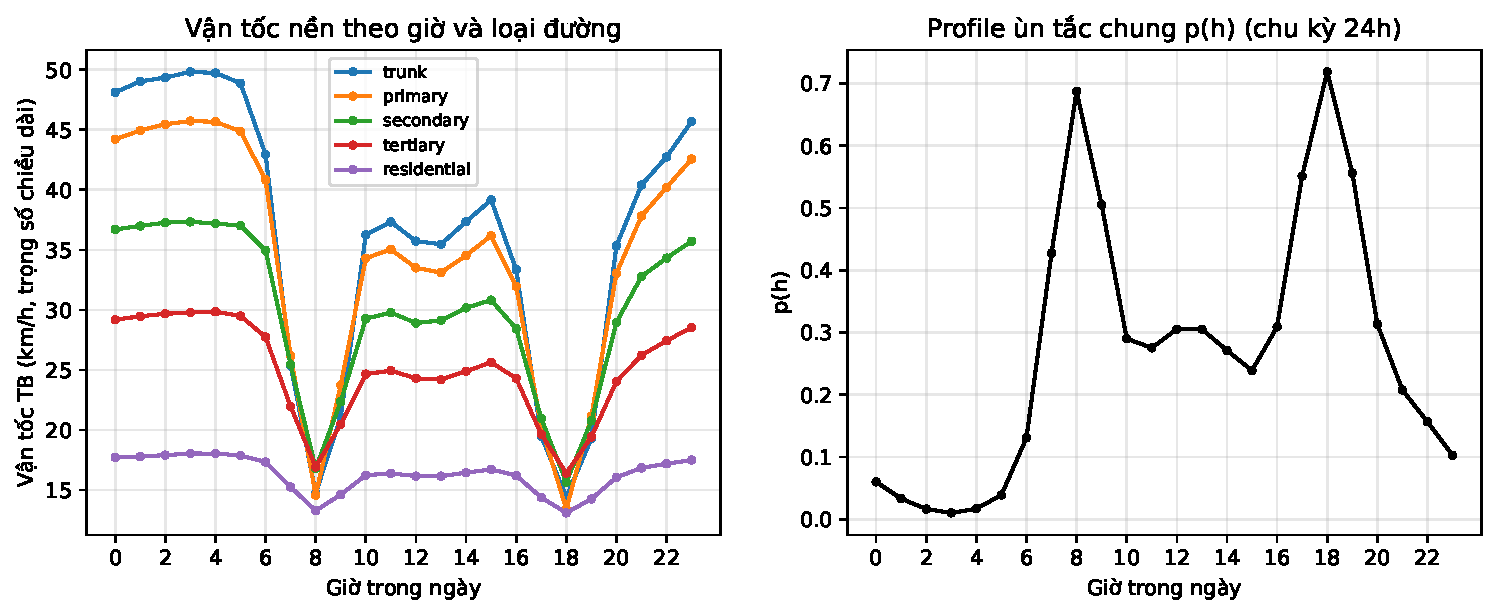
\includegraphics[width=\linewidth]{speed_curves.pdf}
\caption{Vận tốc nền trung bình theo giờ và nhóm đường (trái); profile ùn tắc chung $p(h)$ (phải).}
\label{fig:speedcurves}
\end{figure}

\begin{figure}[H]
\centering
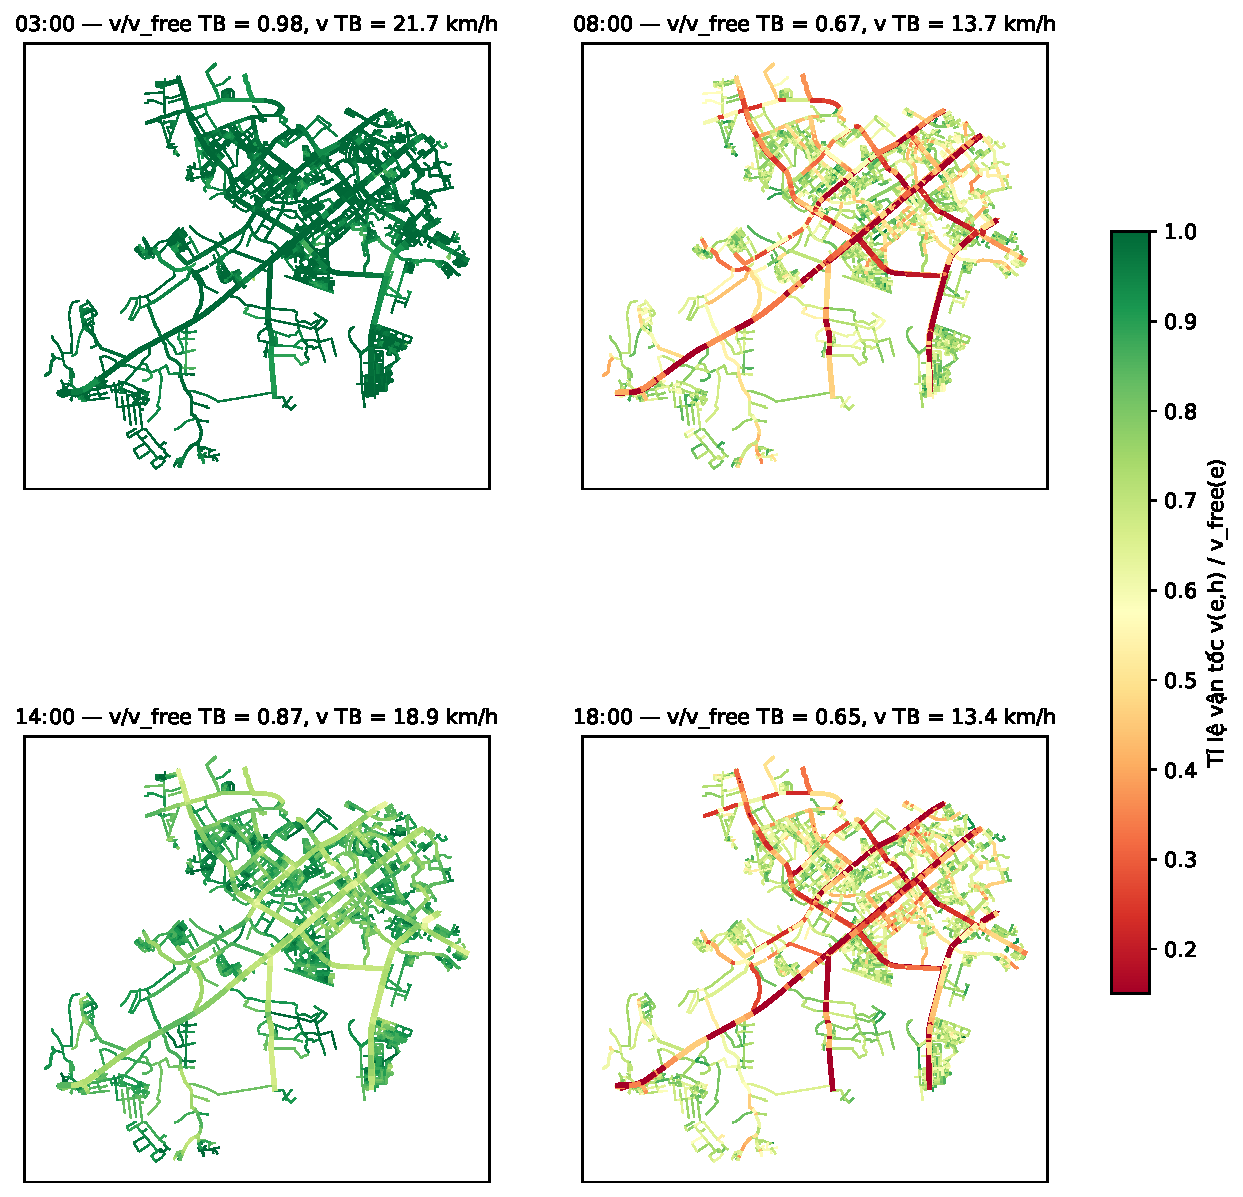
\includegraphics[width=0.82\linewidth]{speed_maps.pdf}
\caption{Tỉ lệ $v/v_{\text{free}}$ trên toàn mạng lúc 3h, 8h, 14h và 18h.}
\label{fig:speedmaps}
\end{figure}

Hình~\ref{fig:speedcurves} và Hình~\ref{fig:speedmaps} cho thấy mô hình tái hiện đúng các hiện tượng mong muốn: vận tốc
trung bình (trọng số theo chiều dài) là \VThree{} km/h lúc 3h, \VEight{} km/h lúc 8h, \VFourteen{} km/h lúc 14h và
\VEighteen{} km/h lúc 18h; vào giờ cao điểm các trục chính chuyển sang màu đỏ.

\subsubsection{Môi trường thực với nhiễu tương quan}\label{sec:method:noise}

Môi trường thực của mỗi truy vấn được sinh từ vận tốc nền và một trường nhiễu nhân:
\begin{equation}
V_{\text{real}} = \mathcal{F}\Bigl(V_{\text{base}}\odot \exp\bigl(\sigma Z\bigr)\Bigr),
\label{eq:vreal}
\end{equation}
trong đó $\mathcal{F}$ là thủ tục sửa FIFO \eqref{eq:fifo-fix}, $\odot$ là tích từng phần tử, $\sigma$ là mức nhiễu của
truy vấn (nhận một trong các giá trị $0{,}05$; $0{,}15$; $0{,}30$). Trường $Z$ có phân phối biên chuẩn tắc $\mathcal{N}(0,1)$ nên hệ số $\varepsilon=e^{\sigma Z}$
tuân theo phân phối LogNormal$(0,\sigma)$; nhưng khác với nhiễu độc lập, $Z$ có \emph{tương quan không gian--thời gian}:
\begin{equation}
Z_{\cdot,h} = \rho\, Z_{\cdot,h-1} + \sqrt{1-\rho^2}\; \hat{A}^{\,k} W_{\cdot,h}, \qquad W_{e,h}\sim\mathcal{N}(0,1),
\label{eq:ar1}
\end{equation}
sau đó chuẩn hoá và trộn với một phần nhiễu độc lập:
\begin{equation}
Z \leftarrow \sqrt{1-\gamma}\; Z + \sqrt{\gamma}\; U, \qquad U_{e,h}\sim\mathcal{N}(0,1),
\label{eq:mix}
\end{equation}
với $\rho=\NoiseRho$, $k=4$, $\gamma=\NoiseIid$. Đo trên trường mẫu, tương quan giữa hai giờ liền kề là \NoiseLagCorr{}
và giữa hai cạnh nối tiếp là \NoiseAdjCorr. Tương quan này là điều kiện để quan sát ở hiện tại và ở lân cận mang thông
tin về tương lai gần và về các cạnh chưa quan sát --- tiền đề của dự báo ngắn hạn ở Mục~\ref{sec:method:gcn}.

\subsubsection{Tìm kiếm phụ thuộc thời gian và heuristic}\label{sec:method:search}

\textbf{TD-Dijkstra} gán cho mỗi nút nhãn $\text{arr}(v)$ là thời điểm đến sớm nhất đã biết. Khi lấy nút $u$ ra khỏi hàng
đợi, mỗi cạnh $e=(u,v)$ được ``nới lỏng'':
\begin{equation}
\text{arr}(v) \leftarrow \min\Bigl(\text{arr}(v),\; \text{arr}(u) + \tau_e\bigl(\text{arr}(u)\bigr)\Bigr).
\label{eq:relax}
\end{equation}
\textbf{TD-A*} ưu tiên các nút theo khoá
\begin{equation}
f(v) = \text{arr}(v) + h(v),
\label{eq:astar-key}
\end{equation}
với $h(v)$ là cận dưới của thời gian còn lại tới đích (Thuật toán~\ref{alg:tdastar}). Chúng tôi cài đặt ba heuristic:

\emph{Heuristic chim bay.} Với $v_{\max}$ là vận tốc lớn nhất toàn cục của mô hình (\VMaxGlobal{} km/h với $V_{\text{base}}$):
\begin{equation}
h_{\text{eu}}(v) = 0{,}995\cdot\frac{\text{dist}(v,d)}{v_{\max}}.
\label{eq:h-eu}
\end{equation}

\emph{Heuristic cận dưới chính xác (LB).} Với mỗi cạnh, thời gian nhỏ nhất qua cạnh trong mọi khung giờ là
\begin{equation}
\tau_{\min}(e) = \frac{L_e}{\max_{h} v(e,h)} \le \tau_e(t)\quad\forall t,
\label{eq:taumin}
\end{equation}
(sự cố chỉ làm chậm nên bất đẳng thức vẫn đúng), và heuristic là khoảng cách ngắn nhất trên đồ thị trọng số $\tau_{\min}$:
\begin{equation}
h_{\text{LB}}(v) = d_{\tau_{\min}}(v,d),
\label{eq:h-lb}
\end{equation}
tính bằng một lần Dijkstra ngược từ đích. Đây là heuristic tĩnh chặt nhất có thể xây từ cận dưới theo từng cạnh.

\emph{Heuristic ALT}~\cite{goldberg2005alt}. Chọn $\mathcal{L}$ gồm 8 điểm mốc theo chiến lược ``điểm xa nhất'' trên đồ
thị $\tau_{\min}$, tiền tính $d(\ell,\cdot)$ và $d(\cdot,\ell)$; heuristic theo bất đẳng thức tam giác:
\begin{equation}
h_{\text{ALT}}(v) = \max_{\ell\in\mathcal{L}} \max\Bigl(d(v,\ell)-d(d,\ell),\; d(\ell,d)-d(\ell,v),\; 0\Bigr).
\label{eq:h-alt}
\end{equation}

\emph{Biên dịch JIT.} Cùng thuật toán TD-A* được viết lại cho Numba~\cite{lam2015numba}, chạy trực tiếp trên mảng CSR và
ma trận vận tốc, cho kết quả và số nút mở rộng trùng khớp với bản Python (đã kiểm chứng bằng kiểm thử đơn vị).
Contraction Hierarchies không được cài đặt: ở quy mô vài nghìn nút, TD-A* biên dịch đã chạy dưới một mili-giây mỗi truy
vấn; CH chỉ thật sự cần thiết khi mở rộng ra toàn thành phố.

\subsubsection{Tái lập kế hoạch}\label{sec:method:replan}

\textbf{Replan.} Tại mỗi giao lộ $u$ ở thời điểm $t$, xe đo độ lệch giữa thời gian thực và dự báo cho mọi cạnh trong bán
kính $r=\ReplanRadius$ m:
\begin{equation}
\delta_e = \tau^{\text{real}}_e(t) - \tau^{\text{base}}_e(t), \qquad e\in\mathcal{N}_r(u),
\label{eq:delta}
\end{equation}
ghi nhớ các độ lệch đã đo, giả định chúng \emph{duy trì} trong tương lai gần và lập lại kế hoạch bằng TD-A* trên mô hình
\begin{equation}
\tau^{\text{obs}}_e(t') = \max\Bigl(\tau^{\text{base}}_e(t') + \delta_e,\; \frac{L_e}{v_{\max}}\Bigr).
\label{eq:tau-obs}
\end{equation}
Cộng một hằng số vào hàm thời gian giữ nguyên tính FIFO, còn cận dưới $L_e/v_{\max}$ giữ heuristic chim bay chấp nhận
được. Xe đi cạnh đầu tiên của kế hoạch mới rồi lặp lại (Thuật toán~\ref{alg:replan}).

\textbf{Replan lười.} Chỉ chạy lại tìm kiếm khi có ít nhất một cạnh quan sát mà độ lệch thay đổi đáng kể so với lúc lập
kế hoạch gần nhất:
\begin{equation}
\exists\, e\in\mathcal{N}_r(u):\quad \bigl|\delta_e^{\text{mới}} - \delta_e^{\text{lúc lập}}\bigr| > \theta\,\tau^{\text{base}}_e(t),
\label{eq:lazy}
\end{equation}
với $\theta=\LazyTheta$; ngược lại xe tiếp tục đi theo kế hoạch cũ.

\textbf{D* Lite với chi phí snapshot.} D* Lite~\cite{koenig2002} tìm kiếm ngược từ đích và duy trì hai giá trị cho mỗi nút:
$g(v)$ và giá trị nhìn trước
\begin{equation}
\text{rhs}(v) = \min_{e=(v,w)} \bigl(c(e) + g(w)\bigr), \qquad \text{rhs}(d)=0,
\label{eq:rhs}
\end{equation}
cùng khoá ưu tiên (với $s$ là vị trí hiện tại và $k_m$ là bù trừ tích luỹ khi xe di chuyển)
\begin{equation}
\text{key}(v) = \Bigl(\min\bigl(g(v),\text{rhs}(v)\bigr) + h(s,v) + k_m,\; \min\bigl(g(v),\text{rhs}(v)\bigr)\Bigr).
\label{eq:dstar-key}
\end{equation}
Vì D* Lite đòi hỏi chi phí tĩnh, ta dùng chi phí \emph{snapshot} $c(e)=\tau^{\text{obs}}_e(t_{\text{snap}})$; giữa hai lần
dựng lại, chỉ các cạnh có quan sát mới được cập nhật và D* Lite chỉ sửa phần lời giải bị ảnh hưởng. Toàn bộ chi phí được
dựng lại sau mỗi \DstarRefresh{} phút di chuyển. Đánh đổi: nhanh hơn TD-A* lặp nhưng bỏ qua biến thiên vận tốc trong
tương lai gần.

\subsubsection{Dự báo ngắn hạn bằng mạng tích chập đồ thị}\label{sec:method:gcn}

Giả định có \SensorFrac\% số cạnh được gắn cảm biến (hoặc có xe thăm dò), gồm mọi trục trunk/primary và một phần ngẫu
nhiên các cạnh khác (tổng cộng \NSensors{} cạnh). Tại thời điểm $t$, ta quan sát log-tỉ số vận tốc
\begin{equation}
r_e(t) = \log\frac{v^{\text{real}}_e(t)}{v^{\text{base}}_e(t)} = \log\frac{\tau^{\text{base}}_e(t)}{\tau^{\text{real}}_e(t)}
\label{eq:logratio}
\end{equation}
trên các cạnh có cảm biến và các cạnh trong bán kính quan sát. Đặc trưng đầu vào của cạnh $e$ là
$x_e=[\,r_e\mathbf{1}_e,\ \mathbf{1}_e,\ \text{onehot}(g_e),\ \sin\omega t,\ \cos\omega t,\ c(e,h)\,]$ với $\mathbf{1}_e$ là cờ
``đã quan sát''. Mạng tích chập đồ thị~\cite{kipf2017gcn} trên đồ thị cạnh--cạnh gồm
\begin{equation}
H^{(0)} = \operatorname{ReLU}\bigl(XW_0\bigr), \qquad
H^{(\ell+1)} = \operatorname{ReLU}\Bigl(\hat{A}H^{(\ell)}W_1^{(\ell)} + H^{(\ell)}W_2^{(\ell)}\Bigr),
\label{eq:gcn}
\end{equation}
với 3 lớp ẩn kích thước 32, đầu ra $\hat{y}_e\in\mathbb{R}^2$ là log-tỉ số dự đoán tại hai mốc giờ $h$ và $h+1$. Hàm mất mát
là sai số bình phương trung bình trên mọi cạnh:
\begin{equation}
\mathcal{L}_{\text{GCN}} = \frac{1}{2m}\sum_{e\in E}\bigl\|\hat{y}_e - y_e\bigr\|_2^2,
\label{eq:gcn-loss}
\end{equation}
huấn luyện bằng Adam trên các ``ngày'' mô phỏng có seed độc lập với tập kiểm tra. Với các mốc giờ xa hơn, dự báo tắt dần
theo hệ số tự tương quan:
\begin{equation}
\hat{r}_e(h+k) = \rho^{\,k-1}\,\hat{y}_{e,2}, \qquad k\ge 2,
\label{eq:decay}
\end{equation}
rồi ma trận vận tốc dự báo $V_{\text{base}}\odot e^{\hat r}$ được đưa vào TD-A*. Hai cách dùng: \emph{plan-once + GCN}
(dự báo một lần lúc xuất phát) và \emph{replan + GCN} (cập nhật GCN mỗi \GcnRecompute{} phút; các cạnh vừa quan sát vẫn
dùng độ lệch đo trực tiếp \eqref{eq:delta}). Đối chứng \emph{plan-once + cảm biến} chỉ dùng độ lệch trên chính các cạnh
có cảm biến mà không lan truyền sang cạnh khác.

\subsubsection{Định tuyến theo rủi ro (P90)}\label{sec:method:risk}

Một ``ngân hàng kịch bản'' gồm $M=\RiskM$ ma trận vận tốc được sinh từ cùng mô hình nhiễu \eqref{eq:vreal} với seed độc
lập với tập kiểm tra. Tập ứng viên $\mathcal{C}$ gồm $\RiskK$ tuyến của thuật toán Yen theo thời gian qua cạnh tại giờ xuất
phát, cộng tuyến TD-A* theo dự báo. Phân vị 90\% của mỗi ứng viên được ước lượng bằng phân vị thực nghiệm trên các kịch bản
và chọn
\begin{equation}
\hat{P} = \arg\min_{P\in\mathcal{C}}\; \widehat{Q}_{0.9}\Bigl\{T^{(j)}(P,t_0)\Bigr\}_{j=1}^{M},
\label{eq:risk-est}
\end{equation}
trong đó $T^{(j)}(P,t_0)$ là thời gian đi tuyến $P$ trong kịch bản $j$, được tính vector hoá đồng thời cho cả $M$ kịch bản.

\subsubsection{Học tăng cường}\label{sec:method:rl}

\textbf{Môi trường.} Môi trường chuẩn Gymnasium: tác tử đứng tại một nút và chọn một trong $K=\MaxOutDeg$ khe cạnh ra
(khe trống bị che bằng mặt nạ). Mỗi tập lấy một cặp điểm đi--đến của tập huấn luyện, với giờ xuất phát, seed nhiễu và sự
cố được sinh \emph{mới} để tác tử không học thuộc. Quan sát \emph{cục bộ} gồm vị trí tương đối tới đích (chuẩn hoá 8 km),
khoảng cách chim bay, $\sin/\cos$ của giờ, tỉ lệ số bước đã dùng; và với mỗi khe cạnh ra: cờ hợp lệ, vận tốc quan sát
hiện tại (nhiễu 5\%) chia 60 km/h, chiều dài chia 500 m, cosin góc giữa cạnh và hướng tới đích, cờ ``nút cuối đã thăm''.

\textbf{Phần thưởng.} Khi đi cạnh $e$ mất $\tau$ phút từ nút $u$ tới nút $u'$:
\begin{equation}
\begin{aligned}
r = -\tau + \lambda\,F(u,u') &+ R_{\text{goal}}\,\mathbf{1}[u'=d] \\
&- R_{\text{rev}}\,\mathbf{1}[u'\ \text{đã thăm}] - R_{\text{out}}\,\mathbf{1}[\text{quá số bước}],
\end{aligned}
\label{eq:reward}
\end{equation}
với $R_{\text{goal}}=10$, $R_{\text{rev}}=1$, $R_{\text{out}}=10$, giới hạn số bước bằng $3\times$ số cạnh của tuyến tham chiếu
cộng 20. Thành phần định hình $F$ có hai dạng: theo khoảng cách chim bay (quy ra phút ở 30 km/h), hoặc \emph{theo thế
năng cost-to-go}~\cite{ng1999}:
\begin{equation}
F(u,u') = \Phi(u') - \Phi(u), \qquad \Phi(u) = -\,\text{ctg}_{\text{tự do}}(u),
\label{eq:shaping}
\end{equation}
trong đó $\text{ctg}_{\text{tự do}}(u)$ là thời gian tự do ngắn nhất từ $u$ tới đích. Thông tin toàn cục này chỉ nằm trong
\emph{phần thưởng} lúc huấn luyện; chính sách không quan sát được nó (Mệnh đề~\ref{md:shaping}).

\textbf{Thuật toán học.} MaskablePPO (sb3-contrib) tối ưu hàm mục tiêu cắt xén của PPO~\cite{schulman2017}:
\begin{equation}
\begin{gathered}
\mathcal{L}^{\text{CLIP}}(\theta) = \mathbb{E}_t\Bigl[\min\bigl(\varrho_t(\theta)\hat{A}_t,\;
\operatorname{clip}(\varrho_t(\theta),1-\epsilon,1+\epsilon)\hat{A}_t\bigr)\Bigr],\\[1mm]
\varrho_t(\theta)=\frac{\pi_\theta(a_t\mid o_t)}{\pi_{\theta_{\text{old}}}(a_t\mid o_t)},
\end{gathered}
\label{eq:ppo}
\end{equation}
với $\hat{A}_t$ là ước lượng lợi thế GAE, $\epsilon=0{,}2$, hệ số chiết khấu $0{,}995$; xác suất của hành động bị che bằng
mặt nạ được đặt bằng 0 trước khi chuẩn hoá~\cite{huang2022}. Huấn luyện theo chương trình ba mức~\cite{bengio2009}: mức 1
(cặp điểm gần dưới 2,5 km, không nhiễu) tới 20\% số bước; mức 2 (mọi cặp, có nhiễu) tới 50\%; mức 3 (thêm sự cố).

\textbf{Các biến thể} (Bảng~\ref{tab:rl-variants}):
\begin{itemize}
    \item \emph{RL cục bộ} --- đúng đặc tả ban đầu: quan sát cục bộ, định hình theo khoảng cách chim bay.
    \item \emph{RL + ctg (quan sát)} --- thí nghiệm đối chứng: thêm cost-to-go tự do (thông tin toàn cục tĩnh) vào quan sát.
    \item \emph{RL + định hình ctg} --- quan sát cục bộ, định hình thưởng theo \eqref{eq:shaping}.
    \item \emph{RL cây-GNN} --- quan sát cây lân cận \TreeDepth{} bước ($K+K^2+K^3$ khe, mỗi khe thêm cờ ngõ cụt, cờ quay đầu,
    tiến độ tới đích). Bộ trích đặc trưng truyền thông điệp từ lá lên gốc với trọng số dùng chung giữa các khe cùng tầng:
    \begin{equation}
    \begin{gathered}
    m_D(j) = \phi_D\bigl(x_D(j)\bigr),\\[1mm]
    m_d(j) = \phi_d\Bigl(\bigl[\,x_d(j)\ \|\ \max_{c\in\text{con}(j)} m_{d+1}(c)\,\bigr]\Bigr),\quad d=D-1,\dots,1,
    \end{gathered}
    \label{eq:tree-gnn}
    \end{equation}
    và vector đặc trưng đưa vào chính sách là $[\psi(x_{\text{glob}}),\, m_1(1),\dots,m_1(K)]$ --- mỗi nhánh tầng 1 ứng với
    một hành động, nên chính sách ``nhìn'' được phía sau mỗi cạnh ra tới $D$ bước.
    \item \emph{RL LSTM} --- RecurrentPPO với LSTM~\cite{hochreiter1997lstm} có 128 đơn vị ẩn. Vì sb3-contrib không hỗ trợ mặt nạ
    cho RecurrentPPO, hành động $a$ được ánh xạ thành $a \bmod \deg^+(u)$.
    \item \emph{RL cây-GNN + BC} --- trước khi chạy PPO, chính sách được học bắt chước từ oracle. Dữ liệu thu theo kiểu DAgger
    nhẹ~\cite{ross2011dagger}: thực thi hành động ngẫu nhiên với xác suất 20\%, còn nhãn luôn là cạnh tiếp theo của tuyến
    oracle tính lại từ trạng thái hiện tại. Hàm mất mát là log-likelihood âm:
    \begin{equation}
    \mathcal{L}_{\text{BC}}(\theta) = -\frac{1}{|\mathcal{D}|}\sum_{(o,a^\ast,\mu)\in\mathcal{D}} \log \pi_\theta\bigl(a^\ast\mid o,\mu\bigr),
    \label{eq:bc}
    \end{equation}
    với $\mu$ là mặt nạ hành động; sau đó tinh chỉnh bằng PPO với tốc độ học nhỏ hơn ($10^{-4}$).
    \item \emph{RL lai (RL + tìm kiếm)} --- hành động là hệ số $\beta\in\{0;\,0{,}5;\,1;\,2;\,4\}$ thể hiện mức tin vào quan sát;
    TD-A* lập kế hoạch trên
    \begin{equation}
    \tau^{(\beta)}_e(t) = \max\Bigl(\tau^{\text{base}}_e(t) + \beta\,\delta_e,\; \frac{L_e}{v_{\max}}\Bigr)
    \label{eq:hybrid}
    \end{equation}
    và xe đi cạnh đầu tiên. $\beta=1$ chính là replan, $\beta=0$ là chỉ dùng dự báo, $\beta>1$ là né vùng chậm mạnh tay hơn;
    quan sát gồm 12 đặc trưng tóm tắt (khoảng cách, giờ, thống kê độ lệch quan sát, độ trễ so với kế hoạch). Vì TD-A* luôn
    tìm được đường trên đồ thị liên thông mạnh, tác tử \emph{luôn} tới đích.
\end{itemize}

\begin{table}[H]
\centering\small
\renewcommand{\arraystretch}{1.2}
\caption{Các biến thể học tăng cường (mỗi biến thể huấn luyện với 3 seed).}
\label{tab:rl-variants}
\begin{tabularx}{\linewidth}{>{\raggedright\arraybackslash}p{3.2cm}>{\raggedright\arraybackslash}p{3.3cm}>{\raggedright\arraybackslash}p{2.6cm}X}
\toprule
\textbf{Biến thể} & \textbf{Quan sát} & \textbf{Thuật toán} & \textbf{Điểm khác biệt} \\
\midrule
RL cục bộ & cục bộ ($K$ cạnh ra) & MaskablePPO & đặc tả gốc, định hình chim bay \\
RL + ctg (quan sát) & cục bộ + cost-to-go & MaskablePPO & đối chứng có thông tin toàn cục \\
RL + định hình ctg & cục bộ & MaskablePPO & định hình thưởng theo thế năng \\
RL cây-GNN & cây \TreeDepth{} bước & MaskablePPO + GNN & quan sát rộng hơn \\
RL LSTM & cục bộ & RecurrentPPO & bộ nhớ (không có mặt nạ) \\
RL cây-GNN + BC & cây \TreeDepth{} bước & MaskablePPO + GNN & học bắt chước oracle trước \\
RL lai & 12 đặc trưng tóm tắt & MaskablePPO & RL chọn $\beta$, TD-A* tìm đường \\
\bottomrule
\end{tabularx}
\end{table}

\subsubsection{Chọn giờ xuất phát}\label{sec:method:departure}

Tác tử quyết định ``đi ngay'' hay ``chờ thêm \WaitStep{} phút'' (tối đa \MaxWaits{} lần). Trạng thái gồm khung 30 phút
trong ngày, số lần đã chờ, nhóm khoảng cách và nhóm mức ùn \emph{dự báo} của chính cặp điểm đi--đến
($T^{\text{dự báo}}(t)/T^{\text{tự do}}$) --- thông tin có sẵn tại thời điểm quyết định. Q-learning dạng bảng~\cite{watkins1992}
cập nhật
\begin{equation}
Q(s,a) \leftarrow Q(s,a) + \alpha\Bigl[r + \gamma\max_{a'}Q(s',a') - Q(s,a)\Bigr],
\label{eq:qlearning}
\end{equation}
với phần thưởng $r=-w\Delta$ khi chờ và $r=-T^{\text{oracle}}(t)$ khi đi. Vì $Q$ khởi tạo bằng 0 trong khi mọi phần thưởng
đều âm, các ô ít được ghé sẽ trông ``lạc quan''; khi ra quyết định chúng tôi chỉ tin $Q$ ở những ô đã được cập nhật ít
nhất \DepMinVisits{} lần, ngược lại mặc định đi ngay.

\subsubsection{Mô phỏng nhiều xe}\label{sec:method:multi}

Mỗi tác tử đại diện cho 20 xe, xuất phát ngẫu nhiên trong khung 7:30--8:00. Tải dẫn đường trên mỗi cạnh trong từng khung
15 phút làm chậm cạnh theo hàm BPR \eqref{eq:bpr} với $\alpha=0{,}5$, $\beta=2$ và năng lực theo nhóm đường. Hai chiến lược:
\emph{dẫn đường giống nhau} (mọi xe chạy TD-A* trên dự báo, không biết xe khác) và \emph{phối hợp tuần tự} (lập kế hoạch
lần lượt theo giờ xuất phát, mỗi xe thấy tải của các xe đã lập trước). Thời gian đi thực tế được tính bằng lặp điểm bất
động giữa tải và lịch trình trên các tuyến cố định.

\subsubsection{Ứng dụng minh hoạ và đóng gói}\label{sec:method:app}

Ứng dụng Streamlit (Hình~\ref{fig:app}) cho phép nhấp bản đồ để đặt điểm đi/đến hoặc vị trí sự cố, chọn giờ và phương
pháp (Dijkstra, TD-A*, replan, D* Lite, P90 và các biến thể RL đã huấn luyện), hiển thị bảng thời gian dự kiến/thực tế
cùng các phân vị P10/P50/P90 trên ngân hàng kịch bản, $k$ tuyến thay thế, lớp màu vận tốc (gộp theo 5 lớp màu, có chú
thích), đường cong thời gian đi theo 24 giờ xuất phát kèm dải P10--P90, và một thẻ vẽ toàn bộ \NEdges{} cạnh bằng WebGL.
Toàn bộ dự án được đóng gói bằng Docker (PyTorch bản CPU) và đã được kiểm tra chạy trong container.

\begin{figure}[H]
\centering
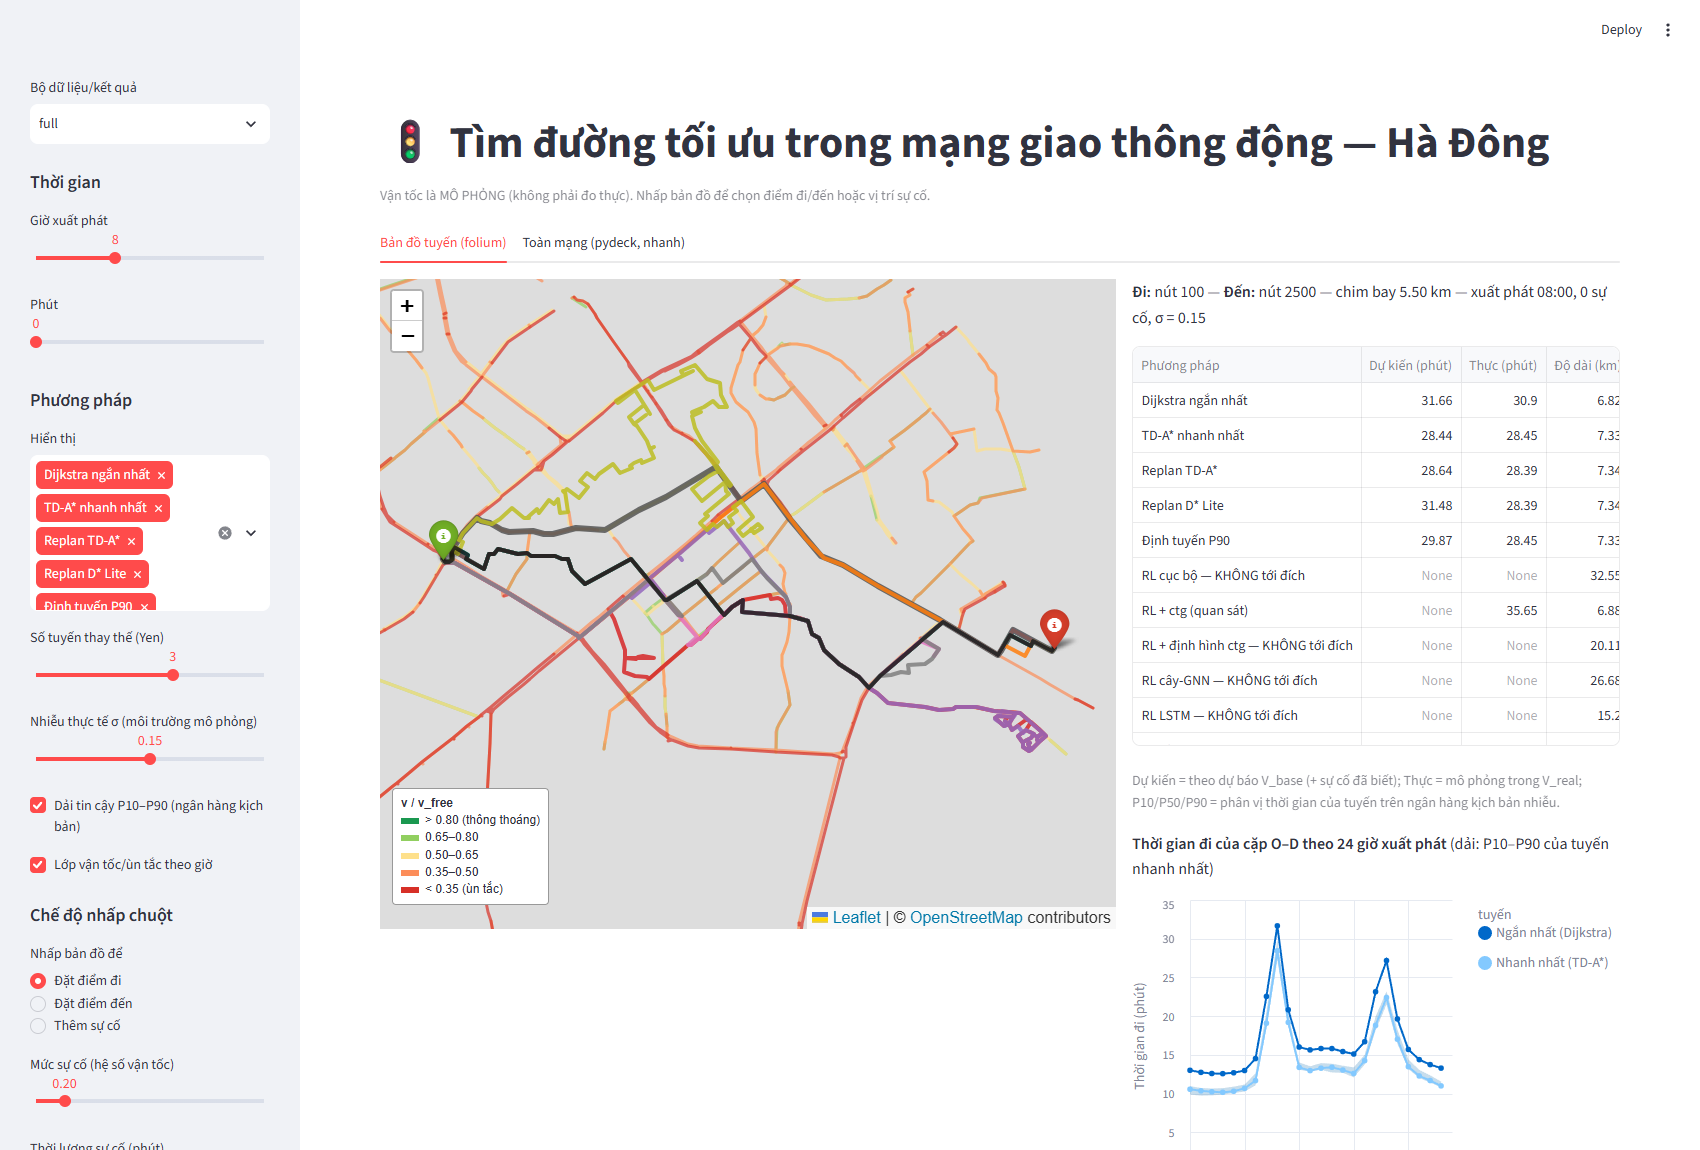
\includegraphics[width=\linewidth]{app_screenshot.png}
\caption{Giao diện ứng dụng minh hoạ (chụp tự động; nền bản đồ không tải trong trình duyệt chạy ẩn).}
\label{fig:app}
\end{figure}

\subsection{Phân tích độ phức tạp / tính đúng đắn}\label{sec:method:correct}

\begin{dl}\label{dl:tdd}
Nếu mọi hàm đến $a_e$ không giảm (FIFO) và $\tau_e(t)>0$, TD-Dijkstra trả về thời điểm đến sớm nhất tại $d$ khi xuất phát từ
$s$ lúc $t_0$.
\end{dl}
\begin{cm}
Gọi $T^\ast(v)$ là thời điểm đến sớm nhất tại $v$. Trước hết, nhờ FIFO, mỗi tiền tố của một đường tối ưu có thể chọn là
tối ưu: nếu đường tối ưu tới $v$ đi qua $x$ ở thời điểm $t_x>T^\ast(x)$, thay tiền tố tới $x$ bằng đường đến $x$ lúc $T^\ast(x)$
rồi đi tiếp cùng dãy cạnh; do mọi $a_e$ không giảm, thời điểm đến $v$ không muộn hơn. Bây giờ quy nạp theo thứ tự lấy nút
ra khỏi hàng đợi: giả sử mọi nút đã đóng có nhãn bằng $T^\ast$. Khi lấy $u$ ra, xét đường tối ưu tới $u$ và nút $y$ đầu tiên
trên đó chưa đóng, với nút liền trước $x$ đã đóng. Khi đóng $x$, cạnh $(x,y)$ đã được nới lỏng nên
$\text{arr}(y)\le a_{xy}(T^\ast(x))=T^\ast(y)\le T^\ast(u)$, bất đẳng thức cuối do $\tau>0$. Vì $u$ được chọn trước $y$ nên
$\text{arr}(u)\le\text{arr}(y)\le T^\ast(u)$; mặt khác $\text{arr}(u)\ge T^\ast(u)$ theo định nghĩa. Vậy $\text{arr}(u)=T^\ast(u)$.
\end{cm}

\begin{md}\label{md:heur}
Các heuristic $h_{\text{eu}}$ \eqref{eq:h-eu}, $h_{\text{LB}}$ \eqref{eq:h-lb} và $h_{\text{ALT}}$ \eqref{eq:h-alt} đều chấp nhận được
và nhất quán: $h(u)\le\tau_e(t)+h(v)$ với mọi $e=(u,v)$ và mọi $t$. Do đó TD-A* trả về lời giải tối ưu và mỗi nút được mở
rộng tối đa một lần.
\end{md}
\begin{cm}
Từ \eqref{eq:taumin} và việc chiều dài cạnh được ép không nhỏ hơn khoảng cách hai đầu:
$\tau_e(t)\ge\tau_{\min}(e)\ge L_e/v_{\max}\ge \text{dist}(u,v)/v_{\max}$. Với $h_{\text{eu}}$: bất đẳng thức tam giác cho
$\text{dist}(u,d)\le\text{dist}(u,v)+\text{dist}(v,d)$. Với $h_{\text{LB}}$: theo định nghĩa khoảng cách ngắn nhất,
$d_{\tau_{\min}}(u,d)\le\tau_{\min}(e)+d_{\tau_{\min}}(v,d)$. Với $h_{\text{ALT}}$: mỗi số hạng trong \eqref{eq:h-alt} là cận dưới
nhất quán theo bất đẳng thức tam giác trên đồ thị $\tau_{\min}$~\cite{goldberg2005alt}, và cực đại của các heuristic nhất
quán vẫn nhất quán. Hệ số an toàn nhỏ hơn 1 chỉ làm $h$ nhỏ đi. Cuối cùng, với $h$ nhất quán, hàng đợi theo khoá
\eqref{eq:astar-key} tương đương TD-Dijkstra trên trọng số rút gọn không âm, nên Định lý~\ref{dl:tdd} áp dụng được.
\end{cm}

\begin{bd}\label{bd:fifofix}
Thủ tục \eqref{eq:fifo-fix} chỉ làm tăng vận tốc, dừng sau hữu hạn bước, và kết quả thoả $-d\tau_e/dt\le\kappa<1$ trên mọi
đoạn, do đó thoả FIFO.
\end{bd}
\begin{cm}
Với $v_u$ cố định, vế phải của \eqref{eq:slope} giảm ngặt khi $v_\ell$ tăng, nên giá trị $x$ trong \eqref{eq:fifo-fix} là
vận tốc nhỏ nhất làm độ dốc bằng $\kappa$; thay $v_\ell$ bằng $\max(v_\ell,x)$ chỉ làm vận tốc tăng. Mỗi lần sửa có thể làm
đoạn kề phía trước vi phạm, nhưng dãy vận tốc ở mỗi ô là không giảm và bị chặn trên bởi vận tốc lớn nhất của các ô kề,
nên thủ tục hội tụ. Khi không còn vi phạm, $-\tau'\le\kappa<1$, tức \eqref{eq:fifo-deriv} thoả.
\end{cm}

\begin{md}\label{md:fifoize}
Hàm $\tilde a$ trong \eqref{eq:fifoize} không giảm, $\tilde a\le a$, và $\tilde a(t)=a(t)$ tại mọi $t$ mà $a$ đã không giảm trên $[t,\infty)$.
\end{md}
\begin{cm}
Với $t_1\le t_2$, tập $\{t'\ge t_2\}\subseteq\{t'\ge t_1\}$ nên $\tilde a(t_1)\le\tilde a(t_2)$. Chọn $t'=t$ cho
$\tilde a(t)\le a(t)$. Nếu $a$ không giảm trên $[t,\infty)$ thì cực tiểu đạt tại $t'=t$. Nội suy tuyến tính giữa các điểm lưới
của một dãy không giảm vẫn là hàm không giảm.
\end{cm}

\begin{md}\label{md:shaping}
Định hình \eqref{eq:shaping} là định hình theo thế năng nên (với hệ số chiết khấu xấp xỉ 1) không làm thay đổi tập chính
sách tối ưu~\cite{ng1999}; tổng định hình trên mọi quỹ đạo từ $s$ tới đích bằng $\lambda\,\text{ctg}_{\text{tự do}}(s)$, không
phụ thuộc đường đi.
\end{md}
\begin{cm}
Tổng $\sum_k \bigl(\Phi(u_{k+1})-\Phi(u_k)\bigr)$ là tổng lồng nhau, bằng $\Phi(d)-\Phi(s)=\text{ctg}(s)$ vì $\text{ctg}(d)=0$.
Hằng số này chỉ phụ thuộc trạng thái đầu nên không làm thay đổi thứ tự giữa các chính sách. Tính chất này được kiểm
chứng bằng kiểm thử đơn vị.
\end{cm}

\textbf{Độ phức tạp.} Với hàng đợi nhị phân và việc tính $\tau_e(t)$ mất $O(1)$, độ phức tạp của các thành phần chính được
tổng hợp trong Bảng~\ref{tab:complexity} (ở đây $m/n\approx\MeanOutDeg$; $L$ là số điểm mốc; $S$ là số giao lộ trên tuyến;
$\ell$, $H$ là số lớp và kích thước lớp ẩn của GCN; $M$, $k$ là số kịch bản và số ứng viên; $N$ là số xe; $I$ là số vòng
lặp điểm bất động).

\begin{table}[H]
\centering\small
\renewcommand{\arraystretch}{1.25}
\caption{Độ phức tạp thời gian và bộ nhớ của các thành phần.}
\label{tab:complexity}
\begin{tabularx}{\linewidth}{>{\raggedright\arraybackslash}p{4.2cm}>{\raggedright\arraybackslash}X>{\raggedright\arraybackslash}p{3.2cm}}
\toprule
\textbf{Thành phần} & \textbf{Thời gian} & \textbf{Bộ nhớ} \\
\midrule
TD-Dijkstra / TD-A* & $O((n+m)\log n)$ mỗi truy vấn & $O(n+m)$ \\
Heuristic LB & $+\,O((n+m)\log n)$ mỗi đích & $O(n)$ \\
Heuristic ALT & tiền xử lý $O(L(n+m)\log n)$; mỗi $h(v)$ là $O(L)$ & $O(Ln)$ \\
Replan / replan lười & $O(S(n+m)\log n)$ / $O(S'(n+m)\log n)$, $S'\le S$ & $O(n+m)$ \\
D* Lite & dựng lại $O((n+m)\log n)$; cập nhật tăng dần chỉ các nút đổi khoá & $O(n+m)$ \\
Suy luận GCN & $O(\ell\cdot\text{nnz}(\hat{A})\cdot H)$ & $O(mH)$ \\
Định tuyến P90 & $O(k\cdot\text{Yen} + M\,k\,|P|)$ & $O(M\,m\cdot 24)$ \\
Mô phỏng nhiều xe & $O(N\cdot\text{TD-A*} + I\,N\,|P|)$ & $O(m\cdot \#\text{khung})$ \\
Chính sách RL & $O(|P|)$ lượt suy luận mạng; biến thể lai thêm một TD-A* mỗi bước & số tham số mạng \\
\bottomrule
\end{tabularx}
\end{table}

\subsection{Lược đồ hoặc sơ đồ minh hoạ}\label{sec:method:diagram}

Hình~\ref{fig:pipeline} là sơ đồ khối luồng dữ liệu của toàn hệ thống. Thuật toán~\ref{alg:tdastar} và
Thuật toán~\ref{alg:replan} là mã giả của hai thành phần tìm kiếm cốt lõi; Thuật toán~\ref{alg:bc} mô tả quy trình huấn
luyện biến thể RL cây-GNN + BC.

\begin{figure}[H]
\centering
\begin{adjustbox}{max width=\linewidth}
\begin{tikzpicture}[font=\footnotesize,
  box/.style={draw, rounded corners, align=center, minimum height=11mm, text width=3.0cm, fill=#1!12},
  box/.default=blue, arr/.style={-{Stealth[length=2mm]}, thick}]
\node[box=gray] (osm)   at (0,0)    {OpenStreetMap\\(OSMnx, Overpass)};
\node[box]      (graph) at (3.8,0)  {Đồ thị CSR\\làm sạch, chuẩn hoá};
\node[box]      (speed) at (7.6,0)  {Vận tốc 24 khung giờ\\$V_{\text{base}}$ + FIFO};
\node[box]      (scen)  at (11.4,0) {Kịch bản cố định\\train / val / test};
\node[box=orange] (real) at (7.6,-2) {Môi trường thực\\nhiễu tương quan + sự cố};
\node[box=green] (search) at (3.8,-4)  {TD-A* (chim bay/LB/\\ALT/Numba), replan,\\lười, D* Lite};
\node[box=green] (fc)     at (7.6,-4)  {Dự báo GCN\\(cảm biến), P90};
\node[box=red]   (rl)     at (11.4,-4) {RL: cục bộ, cây-GNN,\\LSTM, BC, lai $\beta$};
\node[box=red]    (dep)  at (0,-6)    {Chọn giờ (Q-learning)\\nhiều xe (BPR)};
\node[box=violet] (eval) at (7.6,-6)  {Đánh giá: regret, CI,\\Wilcoxon, đơn luồng};
\node[box=violet] (out)  at (7.6,-8)  {Hình, bảng LaTeX, macro,\\báo cáo, ứng dụng};
\draw[arr] (osm) -- (graph);
\draw[arr] (graph) -- (speed);
\draw[arr] (speed) -- (scen);
\draw[arr] (speed) -- (real);
\draw[arr] (real) -- (search);
\draw[arr] (real) -- (fc);
\draw[arr] (real) -- (rl);
\draw[arr] (search) -- (dep);
\draw[arr] (search) -- (eval);
\draw[arr] (fc) -- (eval);
\draw[arr] (rl) -- (eval);
\draw[arr] (dep) -- (eval);
\draw[arr] (scen.east) -- ++(0.35,0) |- (eval.east);
\draw[arr] (eval) -- (out);
\end{tikzpicture}
\end{adjustbox}
\caption{Sơ đồ khối của hệ thống: luồng dữ liệu từ OpenStreetMap tới đánh giá và báo cáo.}
\label{fig:pipeline}
\end{figure}

\begin{algorithm}[H]
\caption{TD-A* (nhãn là thời điểm đến)}\label{alg:tdastar}
\begin{algorithmic}[1]
\Require Đồ thị $G$, nguồn $s$, đích $d$, giờ $t_0$, hàm $\tau_e(t)$, heuristic nhất quán $h$
\Ensure Tuyến đến sớm nhất và thời điểm đến
\State $\text{arr}[s]\gets t_0$; $Q\gets\{(t_0+h(s),s)\}$; $C\gets\emptyset$
\While{$Q\neq\emptyset$}
  \State $(\cdot,u)\gets$ \Call{PopMin}{$Q$}; \textbf{if} $u\in C$ \textbf{then continue}
  \State $C\gets C\cup\{u\}$; \textbf{if} $u=d$ \textbf{then return} truy vết$(\text{pred},d)$, $\text{arr}[d]$
  \For{$e=(u,v)\in\text{out}(u)$ với $v\notin C$}
    \State $t'\gets\text{arr}[u]+\tau_e(\text{arr}[u])$ \Comment{nới lỏng \eqref{eq:relax}}
    \If{$t'<\text{arr}[v]$}
      \State $\text{arr}[v]\gets t'$; $\text{pred}[v]\gets e$; \Call{Push}{$Q,(t'+h(v),v)$}
    \EndIf
  \EndFor
\EndWhile
\end{algorithmic}
\end{algorithm}

\begin{algorithm}[H]
\caption{Replan (tuỳ chọn lười) với quan sát cục bộ và dự báo GCN}\label{alg:replan}
\begin{algorithmic}[1]
\Require $s,d,t_0$; dự báo $\tau^{\text{base}}$; môi trường thực $\tau^{\text{real}}$; bán kính $r$; ngưỡng $\theta$ (chế độ lười)
\State $u\gets s$; $t\gets t_0$; $\Delta\gets\{\}$; $P\gets[\,]$
\While{$u\neq d$}
  \State cần $\gets (P=[\,])$ \Comment{chế độ đầy đủ: luôn đặt cần $\gets$ true}
  \For{mỗi cạnh $e$ có nút đầu cách $u$ không quá $r$}
    \State $\delta\gets\tau^{\text{real}}_e(t)-\tau^{\text{base}}_e(t)$ \Comment{\eqref{eq:delta}}
    \If{$|\delta-\Delta_{\text{lúc lập}}[e]|>\theta\,\tau^{\text{base}}_e(t)$} cần $\gets$ true \EndIf \Comment{\eqref{eq:lazy}}
    \State $\Delta[e]\gets\delta$
  \EndFor
  \If{cần}
    \State $\tau^{\text{base}}\gets$ GCN(cảm biến, quan sát) nếu dùng dự báo GCN \Comment{\eqref{eq:gcn}}
    \State $P\gets$ TD-A*$(u,d,t)$ trên $\tau^{\text{obs}}$ \Comment{\eqref{eq:tau-obs}}
  \EndIf
  \State $e\gets$ \Call{PopFront}{$P$}; $t\gets t+\tau^{\text{real}}_e(t)$; $u\gets\text{head}(e)$
\EndWhile
\State \Return $t-t_0$
\end{algorithmic}
\end{algorithm}

\begin{algorithm}[H]
\caption{Huấn luyện RL cây-GNN + BC}\label{alg:bc}
\begin{algorithmic}[1]
\Require Tập cặp điểm huấn luyện; số tập thu thập $N_{\text{BC}}$; xác suất khám phá $p$
\Ensure Chính sách $\pi_\theta$ (checkpoint tốt nhất theo tập kiểm định)
\State $\mathcal{D}\gets\emptyset$
\For{$i=1,\dots,N_{\text{BC}}$}
  \State Sinh tập mới (cặp điểm, giờ, nhiễu, sự cố); $P\gets$ TD-A* trên $V_{\text{real}}$ \Comment{oracle}
  \While{chưa kết thúc}
    \State $a^\ast\gets$ chỉ số cạnh đầu của $P$; $\mathcal{D}\gets\mathcal{D}\cup\{(o,a^\ast,\mu)\}$
    \State thực thi $a\gets$ ngẫu nhiên hợp lệ với xác suất $p$, ngược lại $a^\ast$
    \State \textbf{if} $a\neq a^\ast$ \textbf{then} $P\gets$ TD-A* lại từ trạng thái mới \textbf{else} bỏ cạnh đầu của $P$
  \EndWhile
\EndFor
\State Cực tiểu $\mathcal{L}_{\text{BC}}$ \eqref{eq:bc} bằng Adam trên $\mathcal{D}$
\State Tinh chỉnh bằng MaskablePPO \eqref{eq:ppo} theo chương trình 3 mức; đánh giá định kỳ trên tập kiểm định, lưu checkpoint tốt nhất
\end{algorithmic}
\end{algorithm}
